\section{Pulverdiffraktometrie}
%kurz das ziel dieses versuchsteiles ansprechen, damit keine zwei �berschriften direkt �bereinander stehen!
%bei schwierigeren versuchen kann auch der theoretische hintergrund erl�utert werden. (mit formeln, herleitungen und erkl�rungen)
Nun soll mit der zuvor verwendeten Methode die Zusammensetzung unbekannter Pulverproben bestimmt werden. Aus den bestimmten Diffraktogrammen soll mittels einer Datenbank die Zusammensetzung bestimmt, so wie die Netzebenabst�nde berechnet werden. Graphisch soll auch die Vertr�glichkeit der gefundenen Kristallstruktur mit dem Diffraktogramm gezeigt werden und die mittlere Kristallgr��e ermittelt werden.
\subsection{Versuchsdurchf�hrung}
Um die Zusammensetzung einer unbekannten Pulverprobe zu bestimmen, werden mit dem Diffraktometer Diffraktogramme erstellt, aus denen mittels einer Datenbank qualitativ die Probenzusammensetzung ermittelt werden kann. Ebenfalls sollen unabh�ngig von der Auswertung mithilfe der Datenbank einige Netzebenenabst�nde d aus den Diffraktogrammen manuell bestimmt werden. Dies geschieht nach der Braggschen Gleichung analog zum Versuchsteil 3.1.2 Formel \ref{eqn:netzebenen}. Nachdem graphisch gezeigt wurde, dass die gefundene Kristallstruktur mit den Diffraktogrammen vertr�glich ist, soll aus den Daten eine Absch�tzung f�r die mittlere Kristallitgr��e gemacht werden, welche aus der Scherrergleichung bestimmt werden kann.
\begin{align}
\delta(2\Theta)_{Korn} = \frac{K \lambda }{B cos{\Theta_0}}
\end{align}
Dabei ist $\delta(2\Theta)$ die volle Halbwertsbreite (FWHM) des Reflexes im Bogenma�, $\Theta_0$ das Maximum des Reflexes, $K$ der Scherrer Formfaktor mit $K \approx 0.94$ (vgl. \cite{scherrer}) und B die gesuchte Korngr��e.
Es ergibt sich f�r die Korngr��e B, wenn man beachtet, dass $E = \frac{hc}{\lambda}$ gilt:
\begin{align}
\label{eqn:scherrer_korngroesse}
B = \frac{0.94 hc}{\delta(2\Theta)_{Korn}Ecos{\Theta_0}}
\end{align}
\subsection{Auswertung}
Bei der Analyse des vorgegebenen Pulvers mittels Debye Scherrer Verfahren ergab sich das Diffraktogramm in Abb. \ref{fig:diffr_pulver}.
Zum Vergleich sind Diffraktogramme von Silicium und Germanium (Abb. \ref{fig:diffr_sil_sim} und Abb. \ref{fig:diffr_ger_sim}) simuliert worden. Man sieht sofort, dass das Diffraktogramm von Silicium mit dem der untersuchten Probe sehr gut �bereinstimmt. Daneben stellt man einen Offset der simulierten Daten zu den gemessenen fest. Um diesen Offset zu bestimmen, wurde an alle drei Datens�tze ein Multivoigt gefittet. Die Voigtverteilung wird dabei numerisch approximiert, wobei die in Python bereits implementierte Voigt-Verteilung aus der Bibliothek "`lmfit"' verwendet wird. Der Fit an die Messdaten passt mit einem reduzierten Chiquadrat von 22,335 relativ gut, wenn man beachtet, dass auch bei kleineren Zahlraten ein Fehler von $\sqrt{N}$ verwendet wurde. Erstaunlicherweise passen die Fits, bei einem Fehler von $\sqrt{N}$, eher schlecht an die simulierten Daten. Man sieht aber, dass die Maxima gut getroffen werden, was in diesem Versuchsteil das wichtigste Kriterium f�r die Auswertung ist. Es ergeben sich reduzierte Chiquadrate von 562 und 19989, sodass diese Fits nicht als besonders gut betrachtet werden k�nnen. Wie die Fits in der N�he einzelner Peaks aussehen, kann im Anhang nachvollzogen werden.
Die Lage der Maxima sind in Tabelle \ref{table:mu_vergleich_pul_si_ger} dargestellt, wobei der Fehler �berall bei $\pm$1 auf der letzten angegebenen Nachkommastelle liegt. Die Fehler ergaben sich aus dem Fit, und wurden nach oben abgesch�tzt.
\begin{table}[H]
\caption{Braggreflexe vom Pulver, verglichen mit den simulierten Daten}
\centering
\label{table:mu_vergleich_pul_si_ger}
\begin{tabular}{|c|c|c|c|c|c|}
\hline  Pulver K$_{\alpha_1}$ & Pulver K$_{\alpha_2}$ & Silicium K$_{\alpha_1}$ & Silicium K$_{\alpha_2}$ & Germanium K$_{\alpha_1}$ & Germanium K$_{\alpha_2}$ \\ 
\hline 2$\theta/^{\circ}$ & 2$\theta/^{\circ}$ & 2$\theta/^{\circ}$ & 2$\theta/^{\circ}$ & 2$\theta/^{\circ}$ & 2$\theta/^{\circ}$ \\ 
\hline 28,287 & 28,363 & 28,447 & 28,521 & 27,317 & 27,389 \\ 
\hline 47,146 & 47,271 & 47,311 & 47,436 & 45,365 & 45,484 \\ 
\hline 55,963 & 56,116 & 56,134 & 56,284 & 53,768 & 53,911 \\ 
\hline 68,969 & 69,167 & 68,144 & 69,340 & 66,096 & 66,282 \\ 
\hline 76,223 & 76,454 & 76,391 & 76,615 & 72,923 & 73,133 \\ 
\hline 87,875 & 88,155 & 88,050 & 88,325 & 83,813 & 84,067 \\ 
\hline 94,802 & 95,111 & 94,975 & 95,285 & 90,214 & 90,499 \\ 
\hline 106,565 & 106,949 & 106,736 & 107,119 & 100,928 & 101,275 \\ 
\hline 113,949 & 114,388 & 114,122 & 114,563 & 107,525 & 107,915 \\ 
\hline 127,406 & 127,985 & 127,584 & 128,166 & 119,145 & 119,630 \\
\hline 136,766 & 137,505 & 136,943 & 137,671 & 126,764 & 127,335 \\
\hline 
\end{tabular}
\end{table}
Wenn man sich dazu die Diffraktogramme in den Abbildungen \ref{fig:diffr_pulver}, \ref{fig:diffr_sil_sim} und \ref{fig:diffr_ger_sim} anguckt, f�llt auf, dass das Diffraktogramm des untersuchten Pulvers mit dem simulierten Diffraktogramm von Silicium sehr gut �bereinstimmt.\\
Genauer gesagt ist das simulierte Diffraktogramm leicht nach rechts veschoben. Deshalb wurden Differenzplots, bei denen die Peaks nach der Energie von gro� nach klein geordnet sind,  erstellt (Abb. \ref{fig:differenzplot_energie}). In zwei weiteren Plots wurde zus�tzlich zwischen den Peaks K$_{\alpha_1}$, K$_{\alpha_2}$ unterschieden.(Abb. \ref{fig:differenzplot_energie_alpha_1} und \ref{fig:differenzplot_energie_alpha_2})
\begin{figure}[H]
  \centering
 
  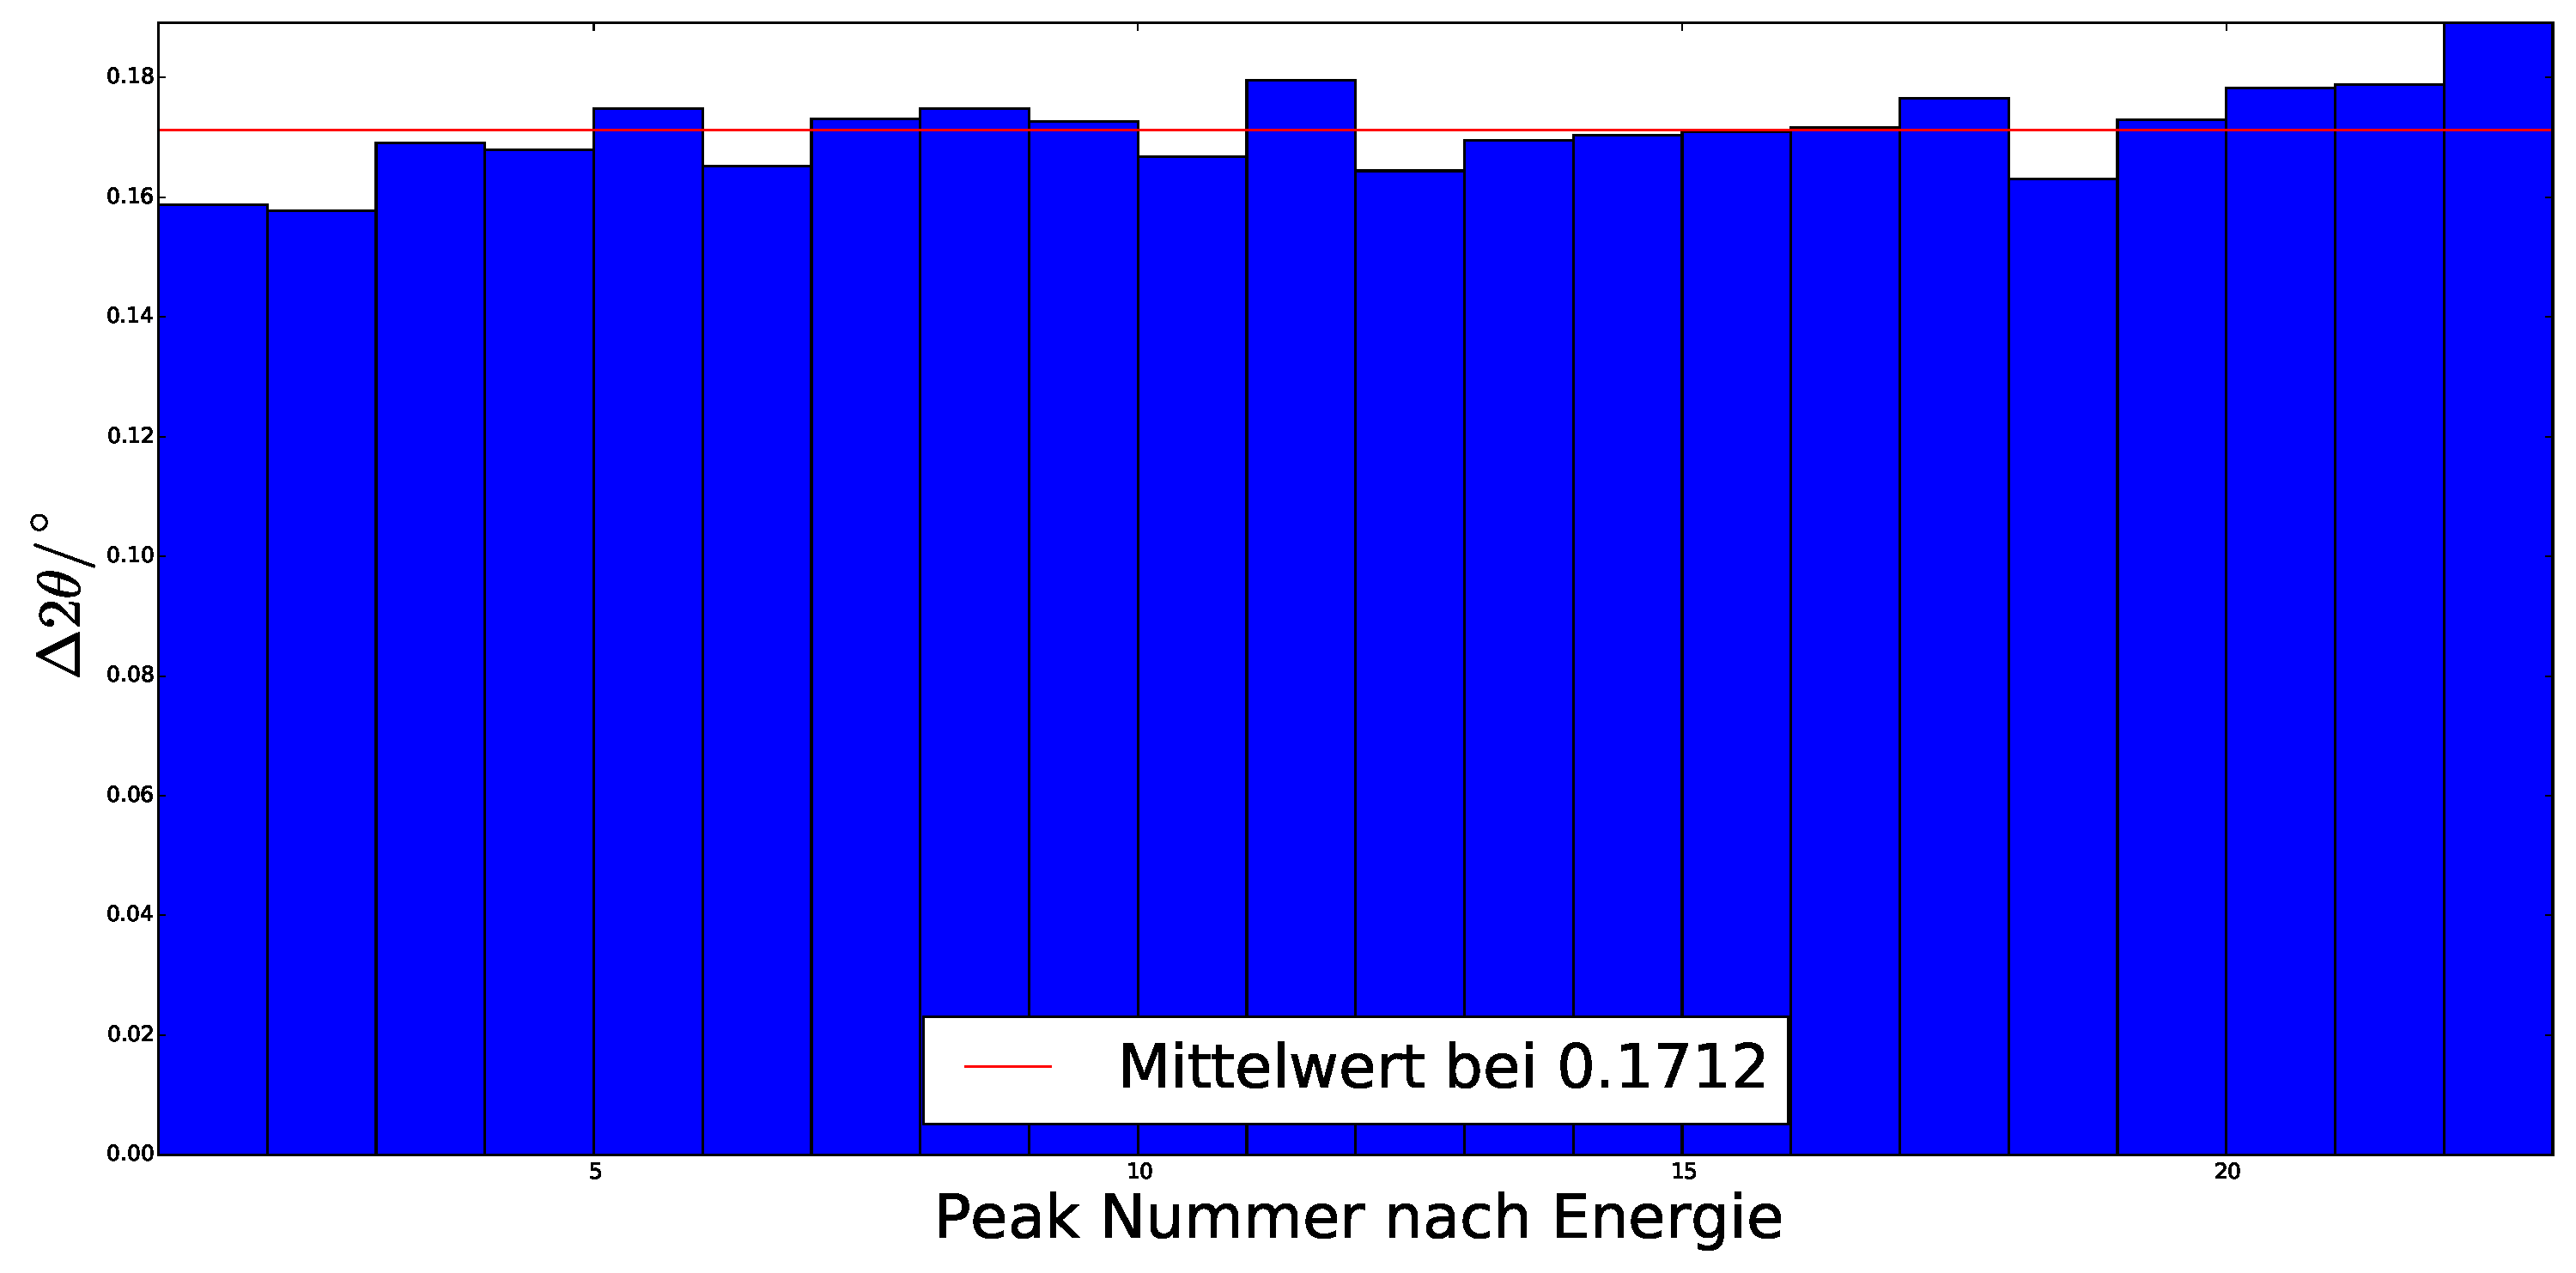
\includegraphics[scale = 0.35]{Differenzplot_pulver_Energie}
   \caption{Peakdifferenzen der Energie nach geordnet} 
  \label{fig:differenzplot_energie}
\end{figure}
\begin{figure}[H]
\begin{minipage}{.49\textwidth}
  \centering
  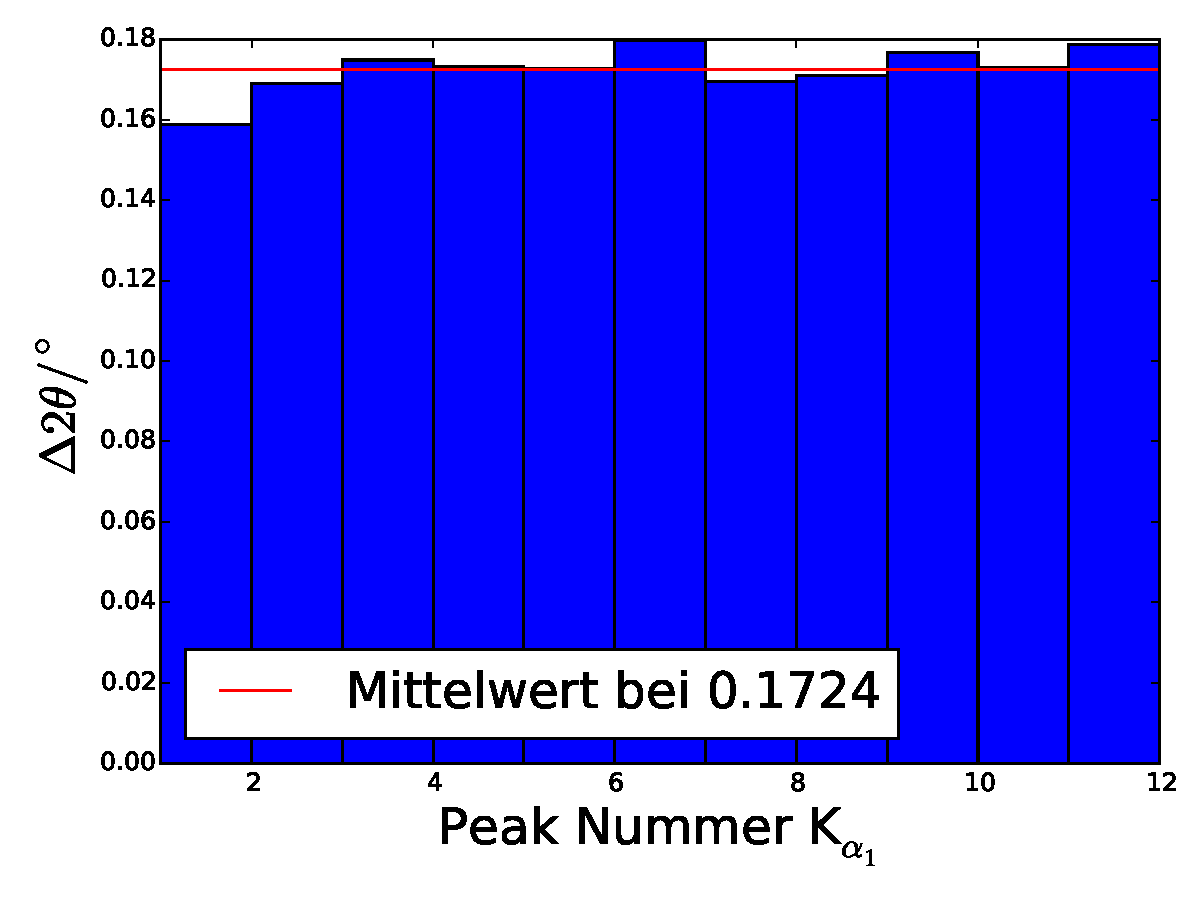
\includegraphics[scale=0.46]{Differenzplot_pulver_K_alpha_1}
  \captionof{figure}{Peakdifferenzen von K$_{\alpha_1}$ der Energie nach geordnet}
  \label{fig:differenzplot_energie_alpha_1}
\end{minipage}
\hspace{0.2cm}
\begin{minipage}{.49\textwidth}
  \centering
  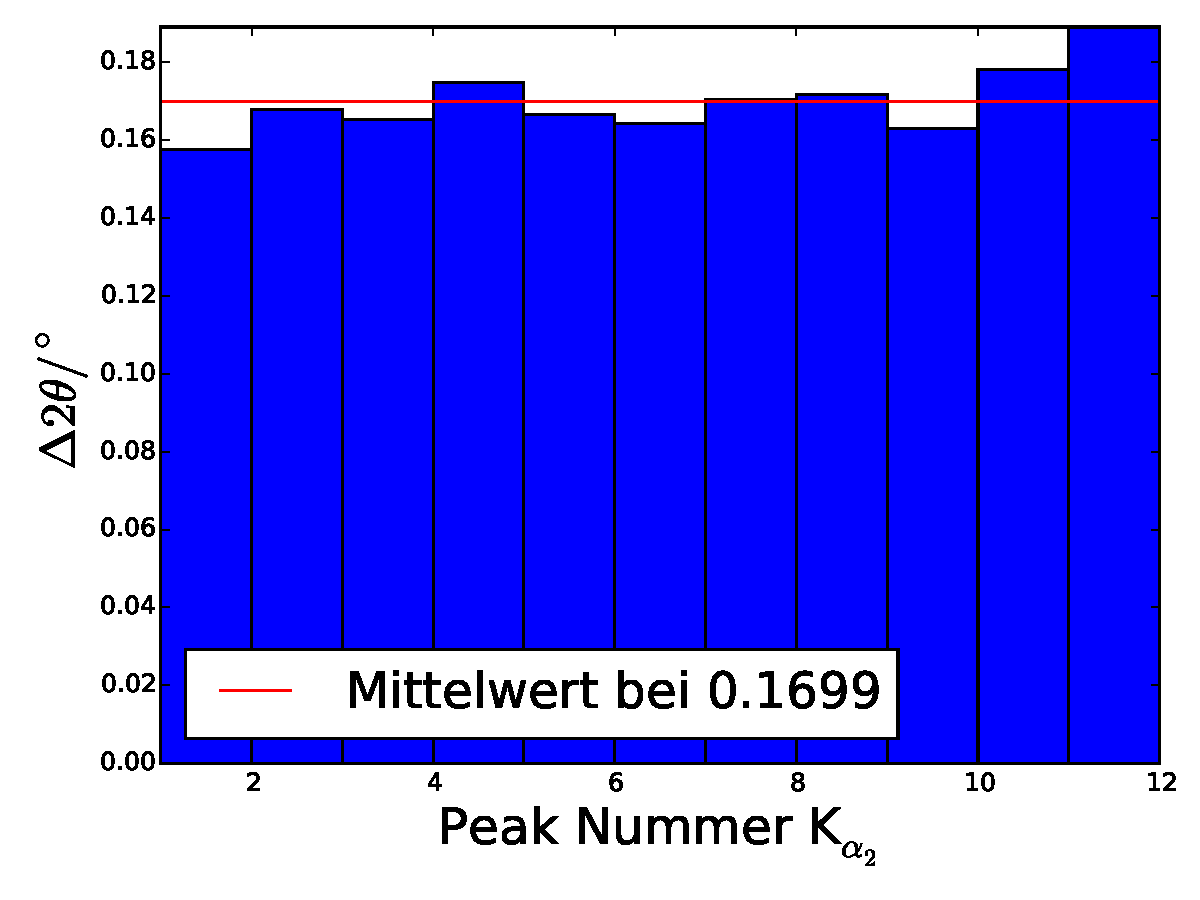
\includegraphics[scale=0.45]{Differenzplot_pulver_K_alpha_2}
  \captionof{figure}{Peakdifferenzen von K$_{\alpha_2}$ der Energie nach geordnet}
  \label{fig:differenzplot_energie_alpha_2}
\end{minipage}
\end{figure}
Man sieht bei allen Plots einen leichten Anstieg der Differenzen der Energien f�r kleine Energiewerte. Es wird trotzdem ein Offset in Form einer Konstanten angenommen. Es ergibt sich damit eine mittlere Abweichung von \SI{0.1712}{\degree}, die haupts�chlich auf einen systematischen Fehler zur�ckzuf�hren ist. Nachdem man die Messdaten um diesen Offset nach rechts verschiebt, stimmt die Lage der Peaks des untersuchten Pulvers bis auf die bereits angesprochene minimale Steigung �berein. Das untersuchte Material kann also mit Siliciumpulver identifiziert werden. Die Herkunft des Offsets ist auf die im Vergleich zur Theorie h�heren gemessenen Energien der K$_{\alpha_1}$ und K$_{\alpha_2}$ Linien in Versuchsteil 3.2.3 zur�ckzuf�hren. Indem man Formel \ref{eqn:bragg_kurze_fassung} nach $\theta$ umstellt, Tabelle \ref{tab:enerige_k}) verwendet und die Winkel mit den Winkeln, welche sich aus den Literaturwerten f�r die Energien ergeben, vergleicht, findet man schlie�lich auch einen Grund f�r die bereits angesprochene minimale Steigung. Nachdem man Formel \ref{eqn:bragg_kurze_fassung} bis zur ersten Ordnung taylort und die Differenz zwischen
\begin{align}
\sin(\theta_{Theorie}) = \frac{hc}{2d_{[nh,nk,nl]} E_{Literatur}}
\end{align}
und
\begin{align}
\sin(\theta_{Messung}) &\approx \frac{hc}{2d_{[nh,nk,nl]} E_{Messung}} \\ \notag
&= \frac{hc}{2d_{[nh,nk,nl]}}\left(\frac{1}{E_{Literatur}}-\frac{1}{E^2_{Literatur}}(E_{Messung}-E_{Literatur})\right)
\end{align}
bildet, findet man den Offset
\begin{align}
\Delta\theta \approx \sin(\theta_{Messung})-\sin(\theta_{Theorie}) \approx \frac{(-1)hc}{2d_{[nh,nk,nl]}E^2_{Literatur}}(E_{Messung}-E_{Literatur})
\end{align}
welcher abh�ngig von d$_{[nh,nk,nl]}$ ist. Bei gro�en Netzebenenabst�nden (kleinen Winkeln $\theta$) ergibt sich ein kleinerer negativer Offset, sowie bei kleinen Netzebenenabst�nden (gr��eren Winkeln $\theta$) ein gr��erer negativer Offset. Die Steigung des Offsets ist gering, da die Unterschiede zwischen den Netzebenenabst�nden gering sind.  Ein konstanter Offset ist deshalb f�r die qualitative Betrachtung ausreichend. Die Netzebenenabst�nde lassen sich aus Formel \ref{eqn:netzebenen} und den in Tabelle \ref{tab:enerige_k} bestimmten Energien bestimmen. Zuvor werden die Ordnung und die Werte h,k,l in der Form [nh,nk,nl] bestimmt, indem man Formel \ref{eqn:d_nh,nk,nl}
\begin{align}
d_{[nh,nk,nl]} = \frac{a}{\sqrt{(nh)^2+(nk)^2+(nl)^2}}
\label{eqn:d_nh,nk,nl}
\end{align}
in Formel \ref{eqn:bragg_kurze_fassung} einsetzt und nach $(nh)^2+(nk)^2+(nl)^2$ umstellt.($a = \SI{5,431020504}{\angstrom}$ ist die Gitterkonstante von Silicium.) Dabei wird auf eine Fehlerrechnung verzichtet.
Es ergibt sich Formel \ref{eqn:(nh)^2+(nk)^2+(nl)^2}.
\begin{align}
(nh)^2+(nk)^2+(nl)^2 = \frac{4E^2a^2}{h^2c^2}\sin^2(\theta)
\label{eqn:(nh)^2+(nk)^2+(nl)^2}
\end{align}
Ob man f�r E die theoretischen Energien oder die experimentell bestimmten Energien aus Tabelle \ref{tab:enerige_k} nimmt, �ndert nichts an den Werten $nh$,$nk$,$nl$. (Aus Symmetriegr�nden $h>k>l$.)
In Tabelle \ref{table:Auswertung_K_alpha_1} und \ref{table:Auswertung_K_alpha_1} werden die so bestimmten Werte $[nh,nk,nl]$, sowie die sich aus Formel \ref{eqn:bragg_kurze_fassung} ergebenden Netzebenenabst�nde d$_{[nh,nk,nl] exp}$ dargestellt und mit den theoretischen Netzebenenabst�nden d$_{[nh,nk,nl] theo}$ aus Formel \ref{eqn:d_nh,nk,nl} verglichen. Die Auswahlregeln f�r Diamantgitter werden dabei beachtet ($h$,$k$,$l$ alle ungerade, oder $h$,$k$,$l$ alle gerade und $h+k+l$ durch 4 teilbar).
\begin{table}[H]
\caption{Auswertung der K$_{\alpha_1}$ Linie}
\centering
\label{table:Auswertung_K_alpha_1}
\begin{tabular}{|c|c|c|c|c|}
\hline  2$\theta_{exp}/^{\circ}$  & d$_{[nh,nk,nl] theo}$ & d$_{[nh,nk,nl] exp}$ & Relative Abweichung/\% & [nh,nk,nl] \\
\hline 28,287 & \SI{3,135601}{\angstrom} & \SI{3,150855}{\angstrom} & 0.486 & [1,1,1]\\
\hline 47,146 & \SI{1,920156}{\angstrom} & \SI{1,925180}{\angstrom} & 0.262 & [2,2,0]\\
\hline 55,963 & \SI{1,637514}{\angstrom} & \SI{1,640995}{\angstrom} & 0.213 & [3,1,1]\\
\hline 68,969 & \SI{1,357755}{\angstrom} & \SI{1,359786}{\angstrom} & 0.150 & [4,0,0]\\
\hline 76,223 & \SI{1,245962}{\angstrom} & \SI{1,247479}{\angstrom} & 0.122 & [3,3,1]\\
\hline 87,875 & \SI{1,108602}{\angstrom} & \SI{1,109590}{\angstrom} & 0.089 & [4,2,2]\\
\hline 94,802 & \SI{1,045200}{\angstrom} & \SI{1,045871}{\angstrom} & 0.064 & [3,3,3]/[5,1,1]\\
\hline 106,565 & \SI{0,960078}{\angstrom} & \SI{0,960458}{\angstrom} & 0.040 & [220]\\
\hline 113,949 & \SI{0,918010}{\angstrom} & \SI{0,918297}{\angstrom} & 0.031 & [531]\\
\hline 127,406 & \SI{0,858720}{\angstrom} & \SI{0,858757}{\angstrom} & 0.004 & [6,2,0]\\
\hline 136,766 & \SI{0,828223}{\angstrom} & \SI{0,828156}{\angstrom} & 0.008 & [5,3,3]\\
\hline 
\end{tabular}
\end{table}
\begin{table}[H]
\caption{Auswertung der K$_{\alpha_2}$ Linie}
\centering
\label{table:Auswertung_K_alpha_2}
\begin{tabular}{|c|c|c|c|c|}
\hline  2$\theta_{exp}/^{\circ}$  & d$_{[nh,nk,nl] theo}$ & d$_{[nh,nk,nl] exp}$ & Relative Abweichung/\% & [nh,nk,nl] \\
\hline 28,363 & \SI{3,135601}{\angstrom} & \SI{3,150912}{\angstrom} & 0.488 & [1,1,1]\\
\hline 47,271 & \SI{1,920156}{\angstrom} & \SI{1,925286}{\angstrom} & 0.267 & [2,2,0]\\
\hline 56,116 & \SI{1,637514}{\angstrom} & \SI{1,640896}{\angstrom} & 0.207 & [3,1,1]\\
\hline 69,167 & \SI{1,357755}{\angstrom} & \SI{1,359801}{\angstrom} & 0.151 & [4,0,0]\\
\hline 76,454 & \SI{1,245962}{\angstrom} & \SI{1,247354}{\angstrom} & 0.112 & [3,3,1]\\
\hline 88,155 & \SI{1,108602}{\angstrom} & \SI{1,109467}{\angstrom} & 0.078 & [4,2,2]\\
\hline 95,111 & \SI{1,045200}{\angstrom} & \SI{1,045871}{\angstrom} & 0.064 & [3,3,3]/[5,1,1]\\
\hline 106,949 & \SI{0,960078}{\angstrom} & \SI{0,960467}{\angstrom} & 0.041 & [220]\\
\hline 114,388 & \SI{0,918010}{\angstrom} & \SI{0,918211}{\angstrom} & 0.022 & [531]\\
\hline 127,985 & \SI{0,858720}{\angstrom} & \SI{0,858763}{\angstrom} &  0.005 & [6,2,0]\\
\hline 137,505 & \SI{0,828223}{\angstrom} & \SI{0,828160}{\angstrom} &  0.008 & [5,3,3]\\
\hline 
\end{tabular}
\end{table}
Man sieht, dass die Abweichungen von den theoretischen Netzebenenabst�nden bei unter einem halben Prozent liegen. Die Resultate best�tigen, dass es sich um Siliciumpulver handelt.
Zuletzt sollen die Korngr��en mithilfe der Scherrer-Gleichung abgesch�tzt werden. Mit Gleichung \ref{eqn:scherrer_korngroesse} wird die Korngr��e aus FWHM und den Energien der K$_{\alpha}$-Linien bestimmt. Auf eine Fehlerrechung wird aufgrund der geringen Genauigkeit des Scherrer-Formfaktors verzichtet.
\begin{table}[H]
\caption{Auswertung der K$_{\alpha_1}$ Linie}
\centering
\label{table:korngroesse_K_alpha_1}
\begin{tabular}{|c|c|c|}
\hline  2$\theta_{exp}/^{\circ}$  & FWHM/$^{\circ}$ & B/\AA{}\\
\hline 28,287 & 0.0256 & 58,222 \\
\hline 47,146 & 0.0256 & 61,597 \\
\hline 55,963 & 0.0384 & 42,620 \\
\hline 68,969 & 0.0384 & 45,663 \\
\hline 76,223 & 0.0320 & 57,402 \\
\hline 87,875 & 0.0256 & 78,401 \\
\hline 94,802 & 0.0512 & 41,707 \\
\hline 106,565 & 0.0512 & 47,216 \\
\hline 113,949 & 0.0705 & 37,666 \\
\hline 127,406 & 0.0769 & 42,482 \\
\hline 136,766 & 0.0640 & 61,294 \\
\hline
\end{tabular} 
\end{table}
\begin{table}[H]
\caption{Auswertung der K$_{\alpha_2}$ Linie}
\centering
\label{table:korngroesse_K_alpha_2}
\begin{tabular}{|c|c|c|}
\hline  2$\theta_{exp}/^{\circ}$  & FWHM/$^{\circ}$ & B/\AA{}\\
\hline 28,363 & 0.0320 & 46,701 \\
\hline 47,271 & 0.0192 & 82,372 \\
\hline 56,116 & 0.0320 & 51,308 \\
\hline 69,167 & 0.0256 & 68,744 \\
\hline 76,454 & 0.0256 & 72,045 \\
\hline 88,155 & 0.0320 & 63,028 \\
\hline 95,111 & 0.0513 & 41,933 \\
\hline 106,949 & 0.0577 & 42,262 \\
\hline 114,388 & 0.0641 & 41,790 \\
\hline 127,985 & 0.0513 & 64,538 \\
\hline 137,505 & 0.0897 & 44,599 \\
\hline
\end{tabular} 
\end{table}
Die Korngr��en k�nnen in der Gr��enordnung von 38\AA{} bis 82\AA{} abgesch�tzt werden. 
\begin{sidewaysfigure}
\centering
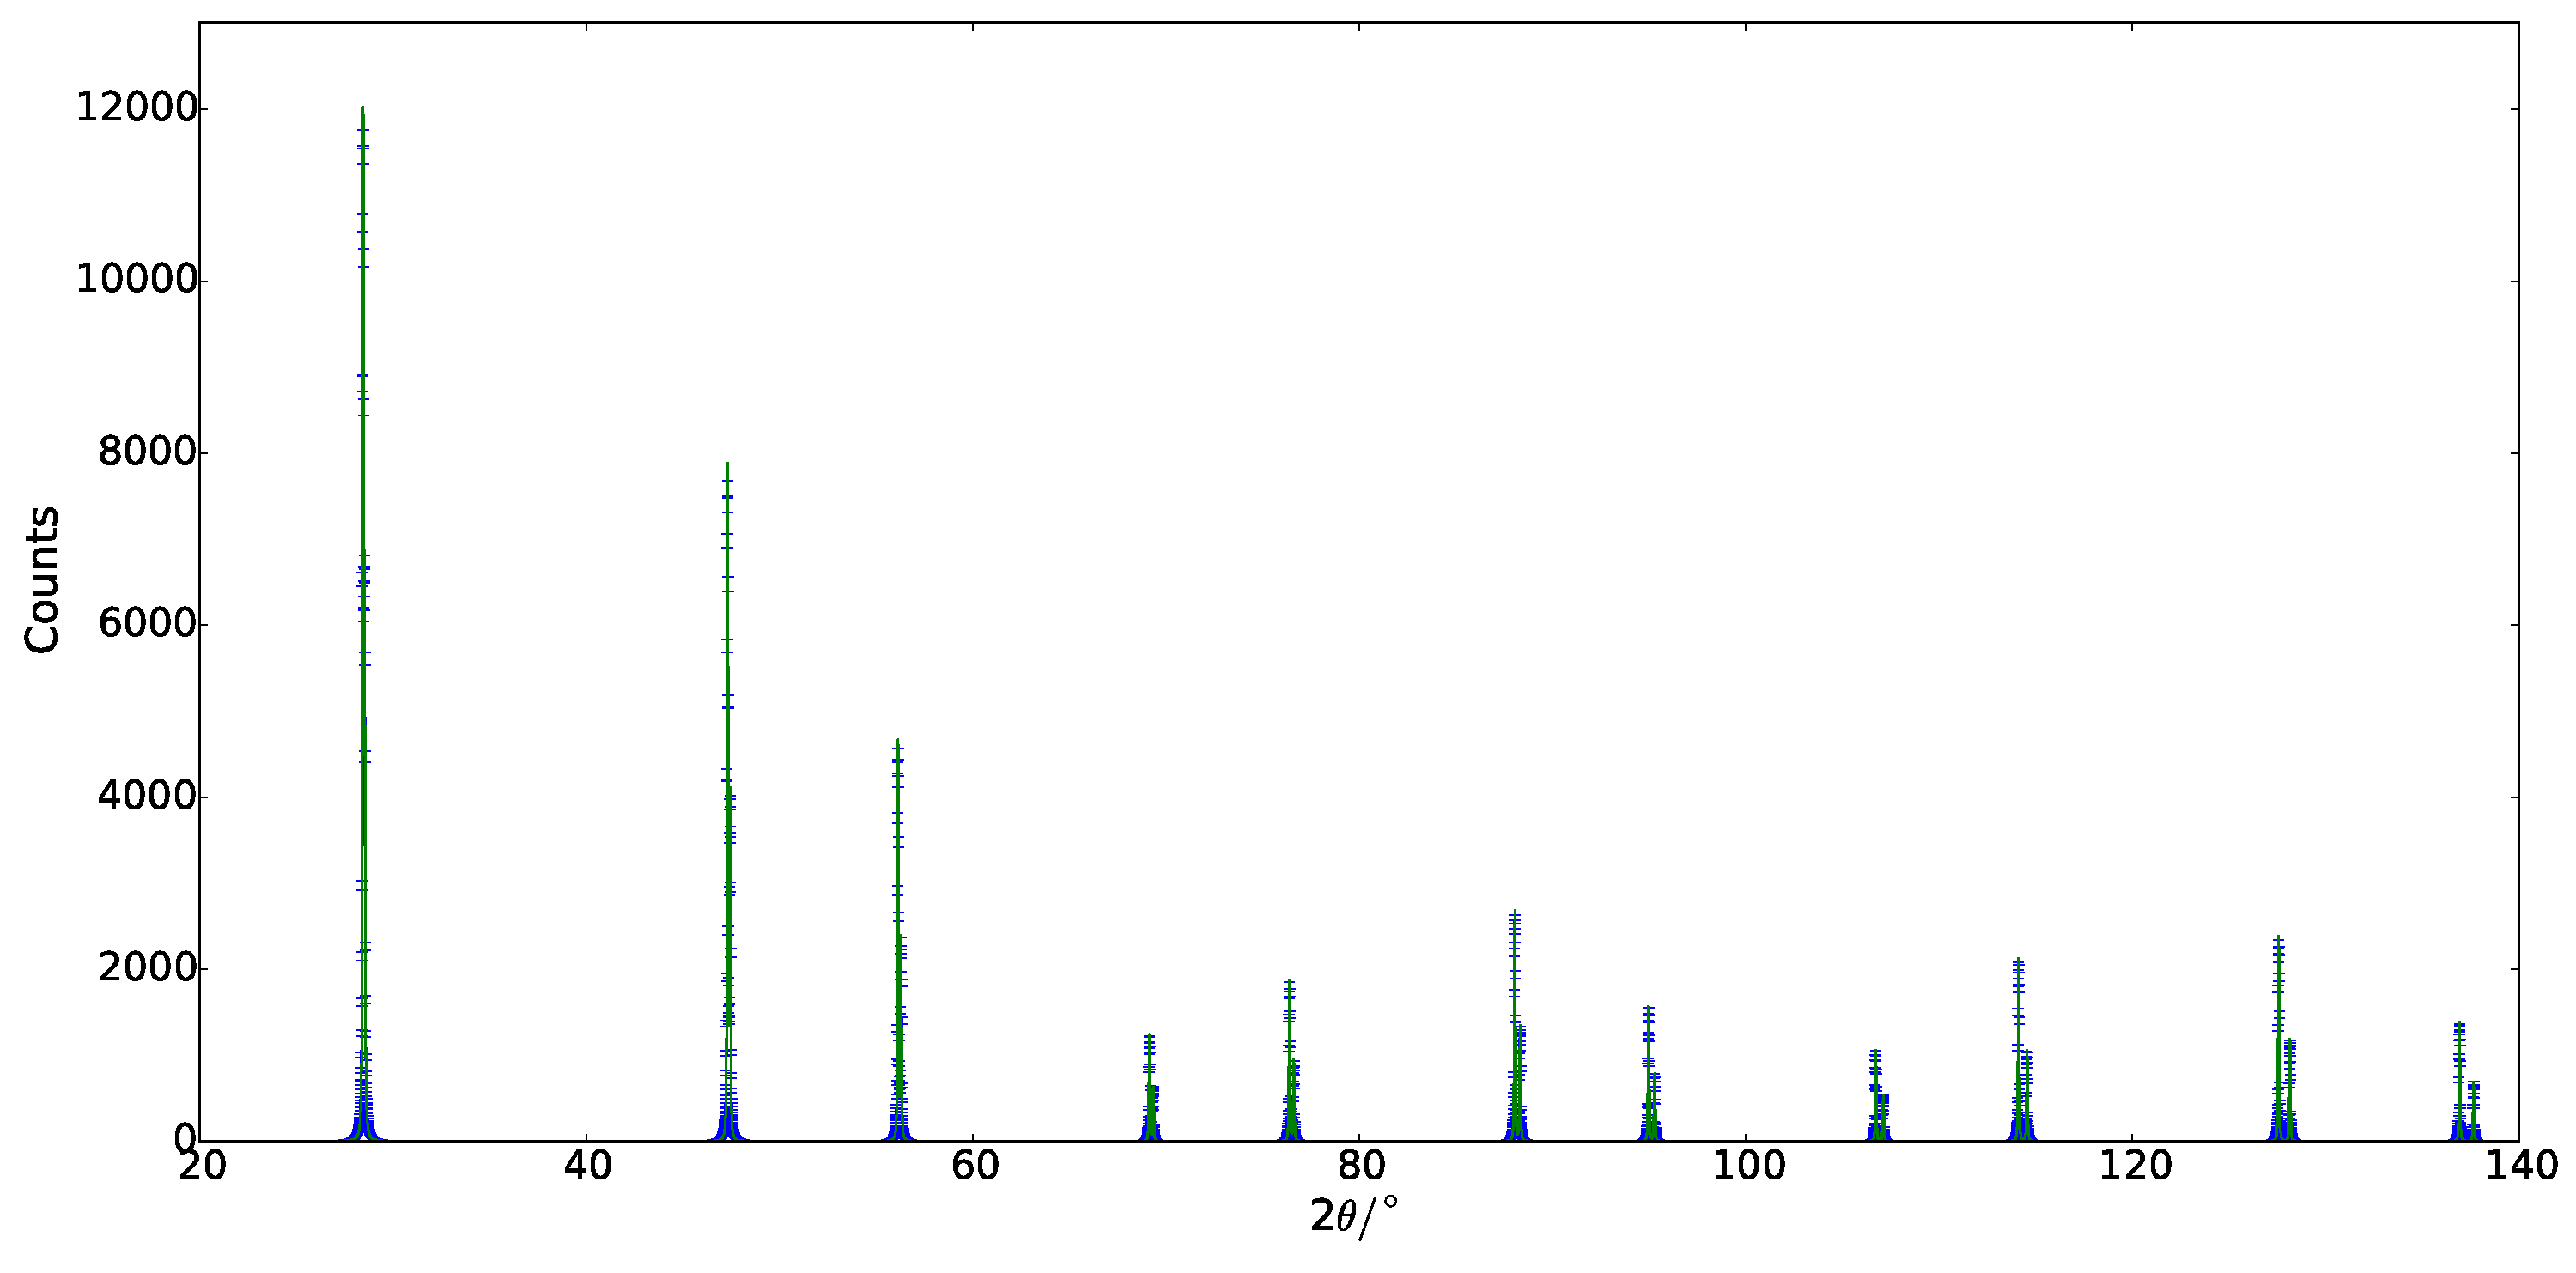
\includegraphics[width = 1.0\textwidth, height = 0.7\textwidth]{messung_pulver_ges}
\caption{Diffraktogramm der Pulverprobe}
\label{fig:diffr_pulver}
\end{sidewaysfigure}
\begin{sidewaysfigure}
\centering
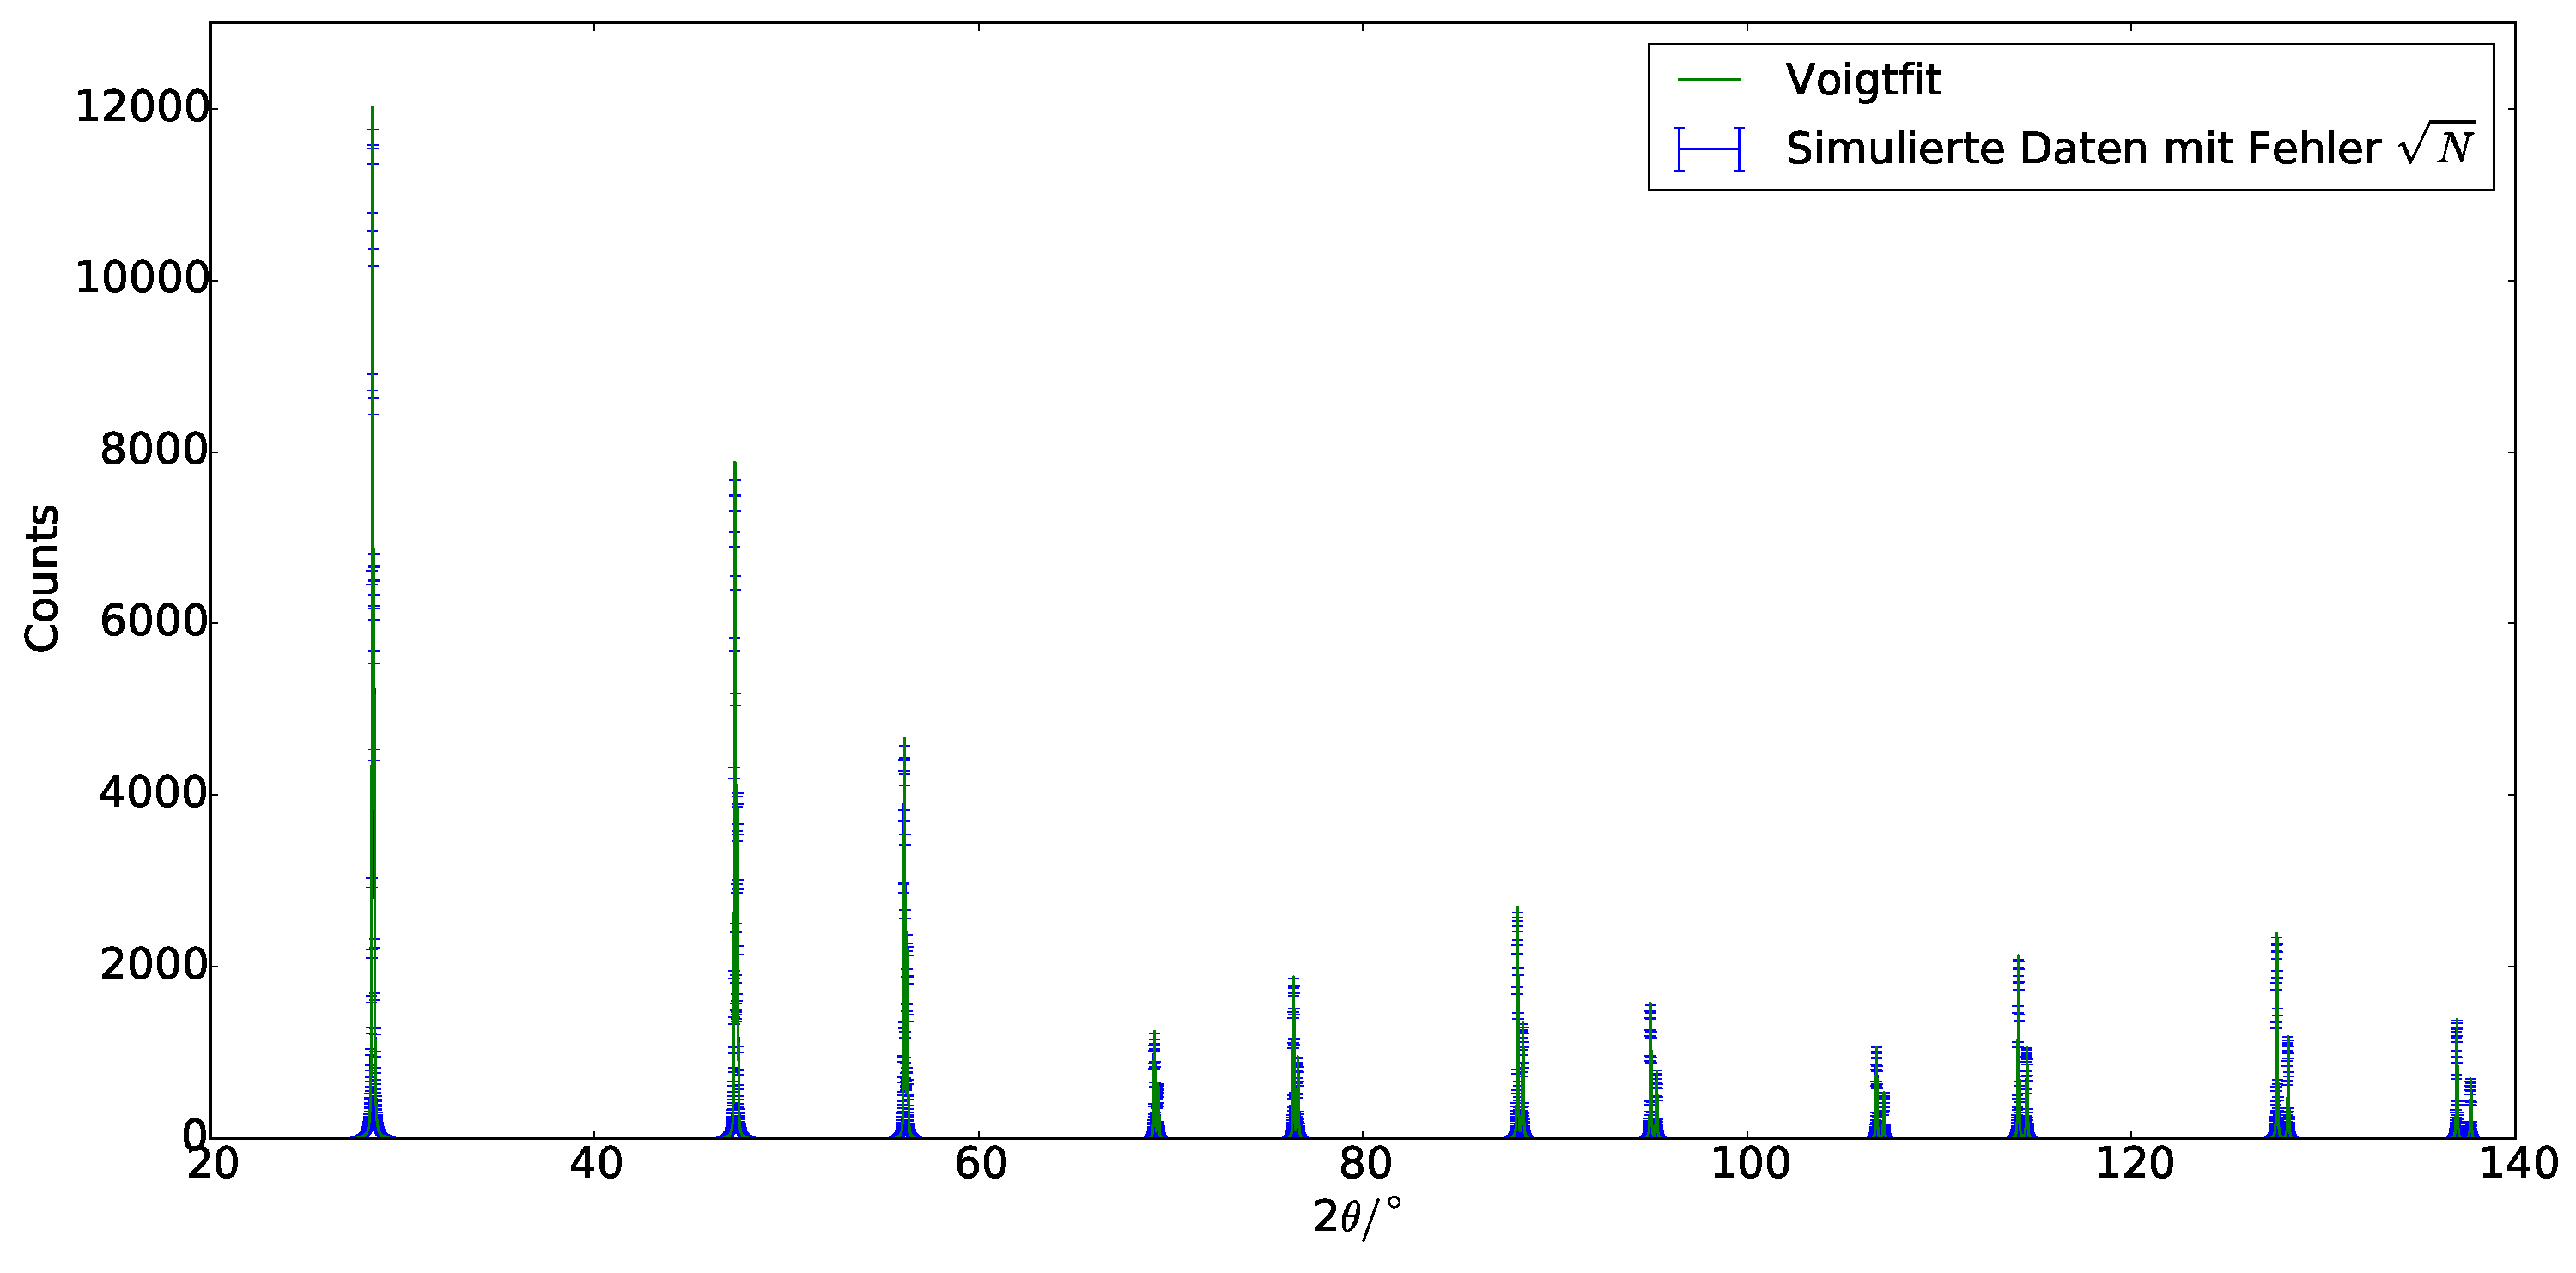
\includegraphics[width = 1.0\textwidth, height = 0.7\textwidth]{Simulation_Siliciumpulver_ges}
\caption{Diffraktogramm der Siliciumsimulation}
\label{fig:diffr_sil_sim}
\end{sidewaysfigure}
\begin{sidewaysfigure}
\centering
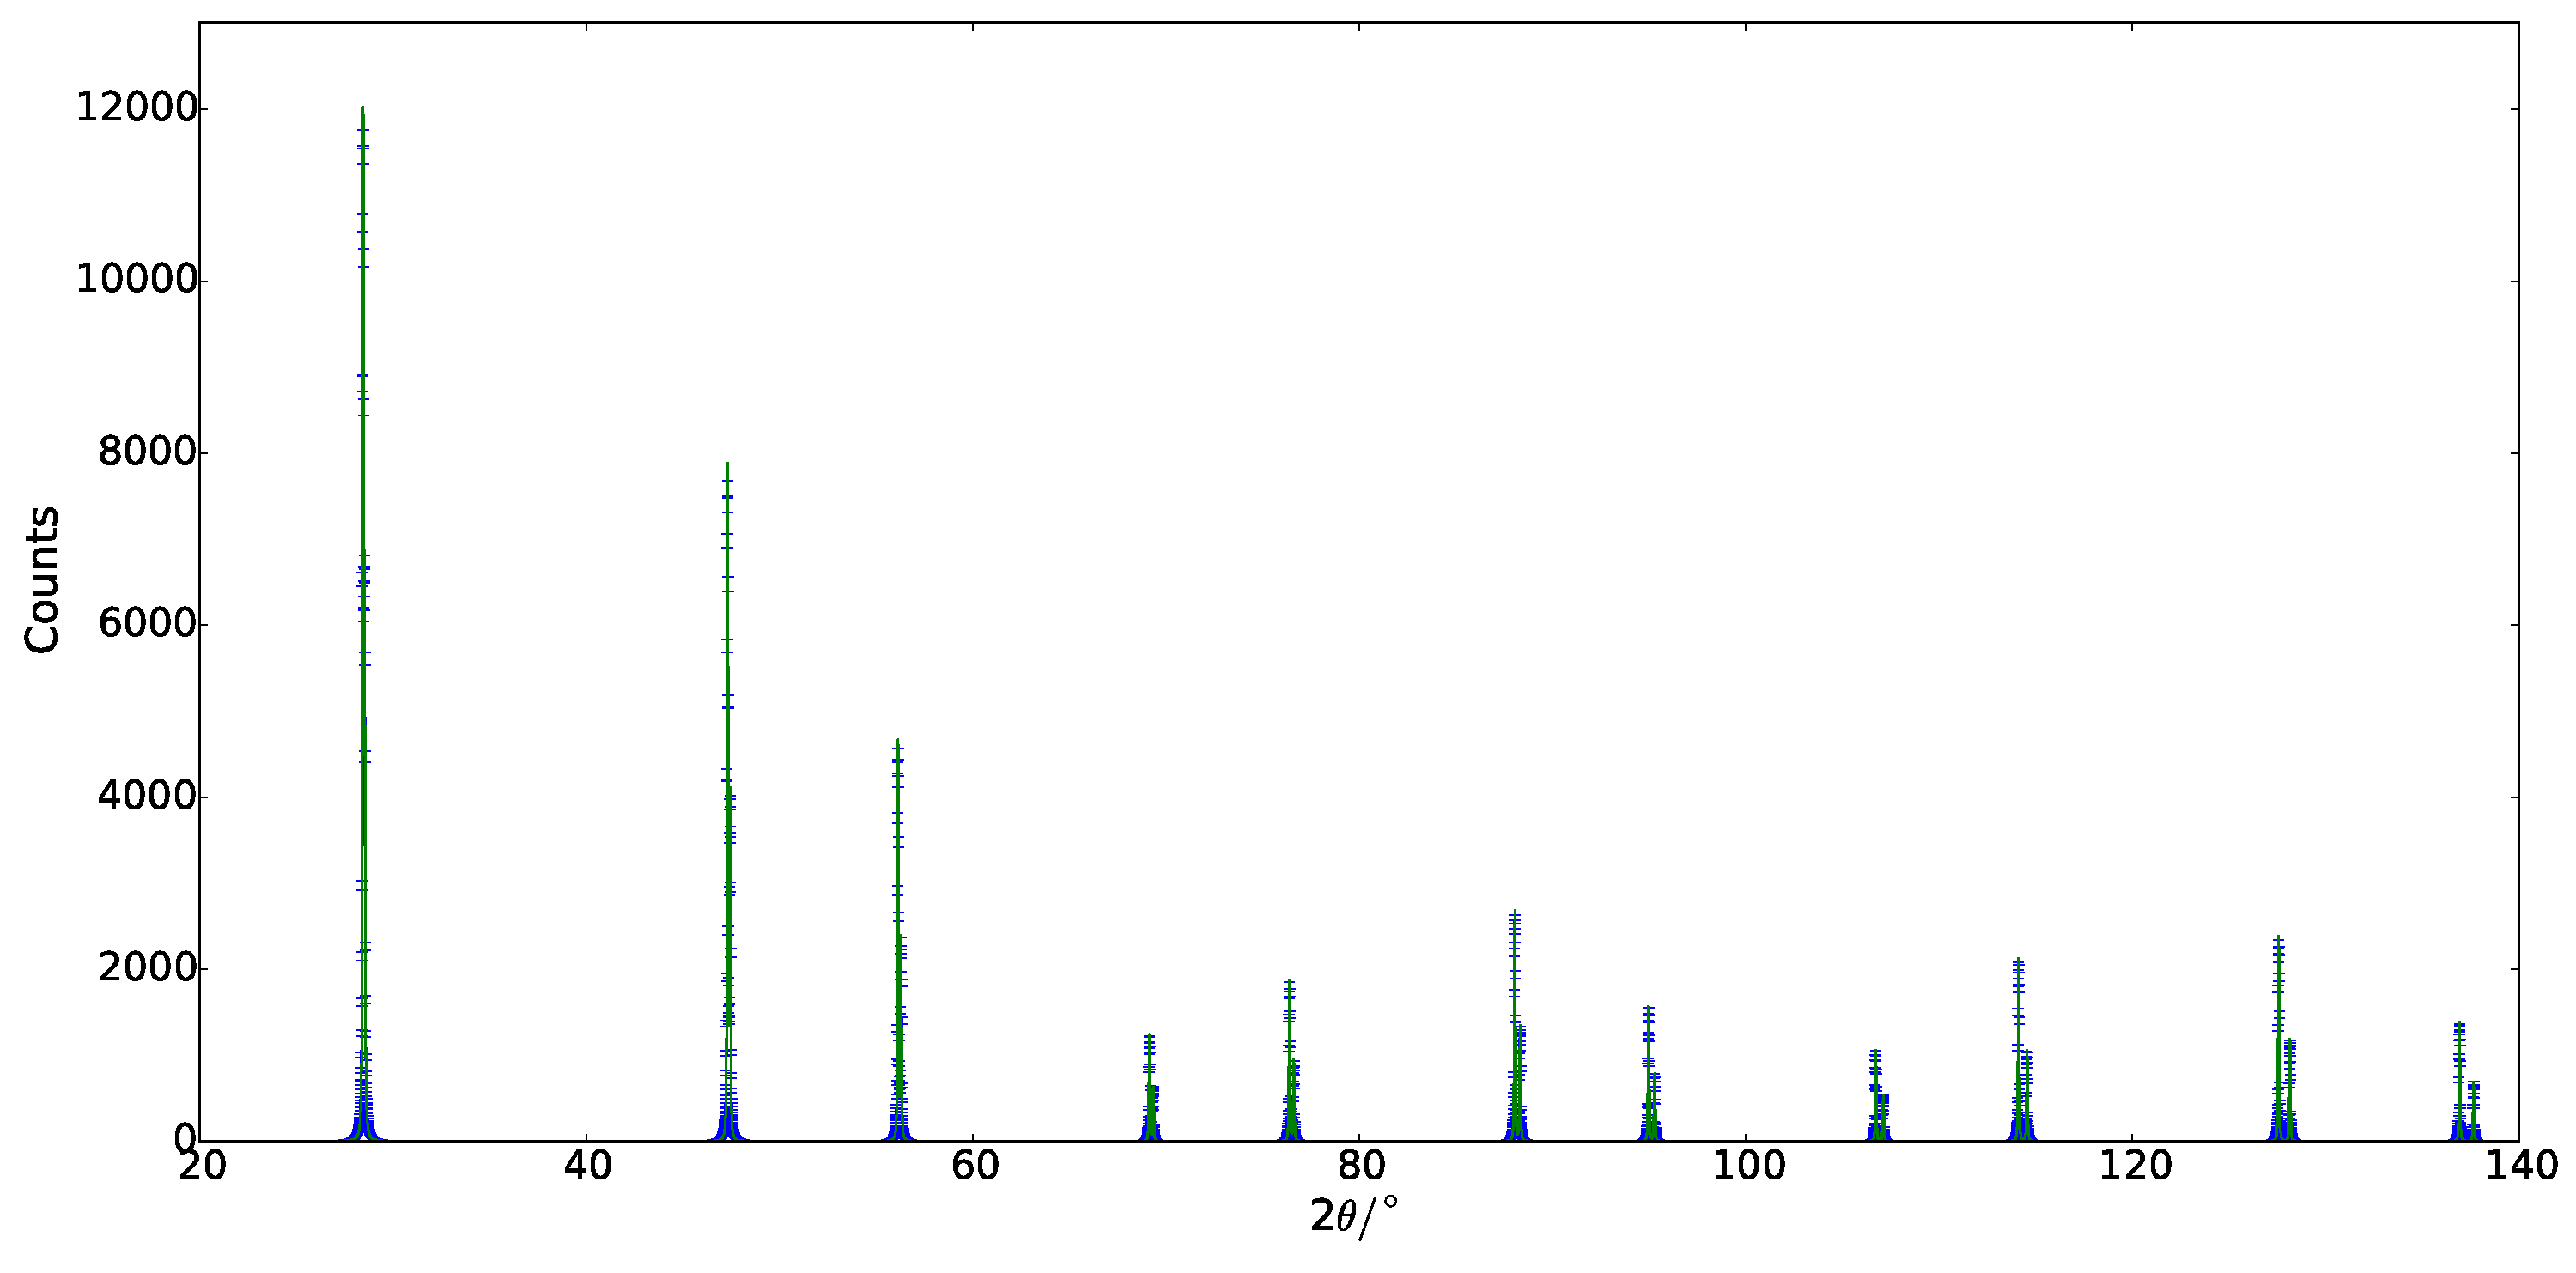
\includegraphics[width = 1.0\textwidth, height = 0.7\textwidth]{messung_pulver_ges}
\caption{Diffraktogramm der Germaniumsimulation}
\label{fig:diffr_ger_sim}
\end{sidewaysfigure}
